\documentclass[12pt]{article}
\usepackage[a4paper, right=1in,top=1.2in,bottom=1.2in,left=1in]{geometry}
\usepackage[utf8]{inputenc}
\usepackage{graphicx}
\usepackage{hyperref}
\usepackage{xcolor}
\usepackage{amsmath}
\usepackage{amssymb}
\usepackage{fancyhdr}
\usepackage{float}
\usepackage{listings}
\usepackage{lmodern}  % for bold teletype font

\usepackage{titlesec}
\titleformat{\section}{\normalfont\Large\bfseries}{}{0pt}{}

\usepackage{tocloft}

\pagestyle{fancy}
\fancyhf{}
\fancyhead[L]{Dhananjay Raman\\Garv Gupta}
\fancyhead[R]{PVR Sai Kumar}
\fancyfoot[C]{\thepage}
\fancyfoot[L]{}

\renewcommand{\headrulewidth}{2pt}
\renewcommand{\footrulewidth}{1pt}

\hypersetup{
colorlinks=true,
linkcolor=red,
filecolor=blue,
urlcolor=red,
}

\definecolor{codegreen}{rgb}{0,0.6,0}
\definecolor{codegray}{rgb}{0.5,0.5,0.5}
\definecolor{codepurple}{rgb}{0.58,0,0.82}
\definecolor{backcolour}{rgb}{0.95,0.95,0.92}

\title{PH556 Project Proposal\\Team Stellar Rulers}
\author{210050044 Dhananjay Raman\\210050120 PVR Sai Kumar\\21D170016 Garv Gupta}
\date{February 2023}

\begin{document}
\maketitle
\tableofcontents
\section{Project Overview}
\begin{itemize}
    \item Target Name: \textbf{V* V471 Vul}
    \item Variability Class: Classical Cepheid Variable
    \item Coordinates (J$2000$): $19^h 34^m 15^s.76\text{ }+19^\circ 34' 14''.6$ ($293.56567\text{ }+19.57072$) \cite{vsx}
    \item Magnitude Range of Target: $14.8 - 15.6$ (in B band) \cite{vsx}
    \item Band of Observation: g
    \item Number of Images Required: $7$
    \item Cadence (Time between two images): $1$ Day
    \item Exposure time: $300$s
    \item Total time of observation: $2100$s
\end{itemize}
\section{Goals}
\begin{itemize}
    \item Our goal is to calculate the period of magnitude oscillation of the target, which is a Classical Cepheid Variable \cite{vsx}.
    \item We will fit this period to a standard Period-Luminosity relationship curve \cite{plrelation} to obtain an empirical absolute magnitude of the target.
    \item Using the apparent magnitude and the calculated absolute magnitude we will then determine the approximate distance to the target.
\end{itemize}
% \textbf{Assumptions:}
% \begin{itemize}
%     \item Target is of type Classical Cepheid Variable.
%     \item Target follows the Period-Luminosity relationship for Classical Cepheids.
%     \item Period of the target is of the order of a few days.
% \end{itemize}
\textbf{Verification:} We will verify our result both using Gaia DR3 \cite{gaia} parallax measurements as well as previous distance calculations \cite{simbad} done from the Period-Luminosity Relationship.
\section{Visibility Plots}
In the months of February the target is visible only for one hour before twilight, and for 2 hours near the end of March. We probably would not be able to take images on the days when the moon is up at this time ($\sim$ 1$^\text{st}$ March - 14$^\text{th}$ March).
\begin{figure}[H]
    \centering
    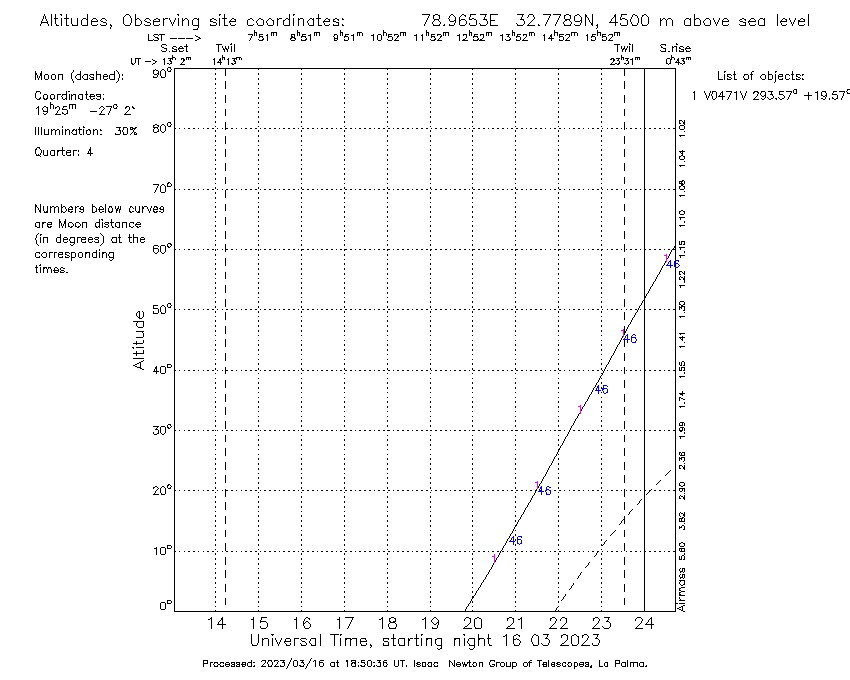
\includegraphics[width=14cm]{16march_visibility.jpg}
    \caption{Visibility on 16 Mar 2023}
    \label{fig:fig1}
\end{figure}
\begin{figure}[H]
    \centering
    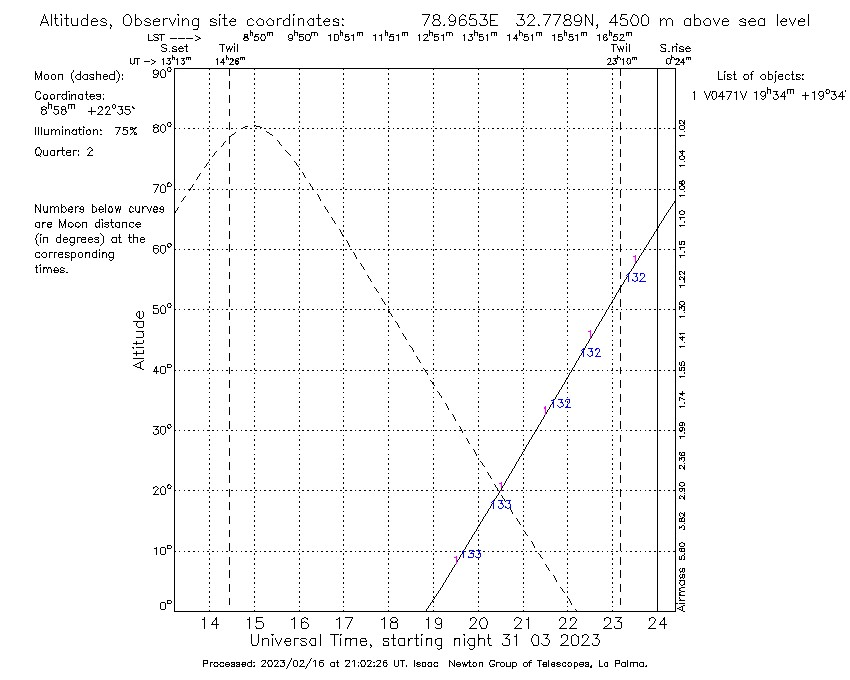
\includegraphics[width=14cm]{31march_visibility.jpg}
    \caption{Visibility on 31 Mar 2023}
    \label{fig:fig2}
\end{figure}
\bibliographystyle{plain}
\bibliography{ref} % Entries are in the refs.bib file
\end{document}